\documentclass[11pt]{article}
\usepackage[margin=1in]{geometry}
\usepackage{amsmath,amssymb,amsthm,bm}
\usepackage{hyperref}
\usepackage{graphicx}
\usepackage{caption}
\usepackage{listings}
\usepackage{xcolor}
\usepackage{float}
\usepackage{placeins}

% Graphics path
\graphicspath{{figures/}}

% Listings style for code
\lstdefinestyle{code}{%
  language=Python,
  basicstyle=\ttfamily\small,
  numbers=left,
  numberstyle=\tiny,
  keywordstyle=\color{blue}\bfseries,
  commentstyle=\color{teal!70!black},
  stringstyle=\color{orange!70!black},
  breaklines=true,
  frame=single,
  rulecolor=\color{black!30},
  tabsize=2,
  showstringspaces=false
}
\lstset{style=code}

\title{k-Nearest Neighbors: Theory and Practice}
\author{}
\date{\today}

\begin{document}
\maketitle

\section{Introduction}
k-Nearest Neighbors (k-NN) is a non-parametric, instance-based learner: predictions are made by looking up the closest training samples. It is simple and often competitive on low-dimensional, well-scaled data, but can be sensitive to feature scaling and suffers in high dimensions.

\section{Theory and Formulas}
Given a query $\mathbf{x}$, find its $k$ nearest neighbors under a distance metric $d(\cdot,\cdot)$ (e.g., Euclidean, Manhattan). For classification, predict by majority vote among the labels of these neighbors; with distance weighting (\texttt{weights=distance}), closer neighbors have higher influence. For regression, predict the average (or distance-weighted average) of neighbor targets.

Computationally, naive search costs $\mathcal{O}(nd)$ per query with $n$ samples and $d$ features. Tree-based indices (KDTree/BallTree) can accelerate queries in moderate dimensions. k-NN is affected by the curse of dimensionality; proper feature scaling and metric choice are critical.

\section{Applications and Tips}
\begin{itemize}
  \item \textbf{Choose k:} tune via cross-validation; odd $k$ helps avoid ties in binary classification.
  \item \textbf{Scaling:} standardize features or use pipelines; scale-sensitive.
  \item \textbf{Metric:} try Euclidean vs Manhattan; consider domain-specific distances.
  \item \textbf{Weights:} \texttt{uniform} vs \texttt{distance}; weighting can help with class overlap.
  \item \textbf{Complexity:} prediction cost grows with data size; consider approximate neighbors for large datasets.
\end{itemize}

\section{Python Practice}
Run the script in this chapter directory to generate figures into \texttt{figures/}.
\begin{lstlisting}[style=code,caption={Generate k-NN figures},label={lst:genfigs_knn}]
python gen_knn_figures.py
\end{lstlisting}

% Include the full Python source
\lstinputlisting[style=code,caption={gen\_knn\_figures.py},label={lst:source_knn}]{gen_knn_figures.py}

\section{Result}
\begin{figure}[H]
  \centering
  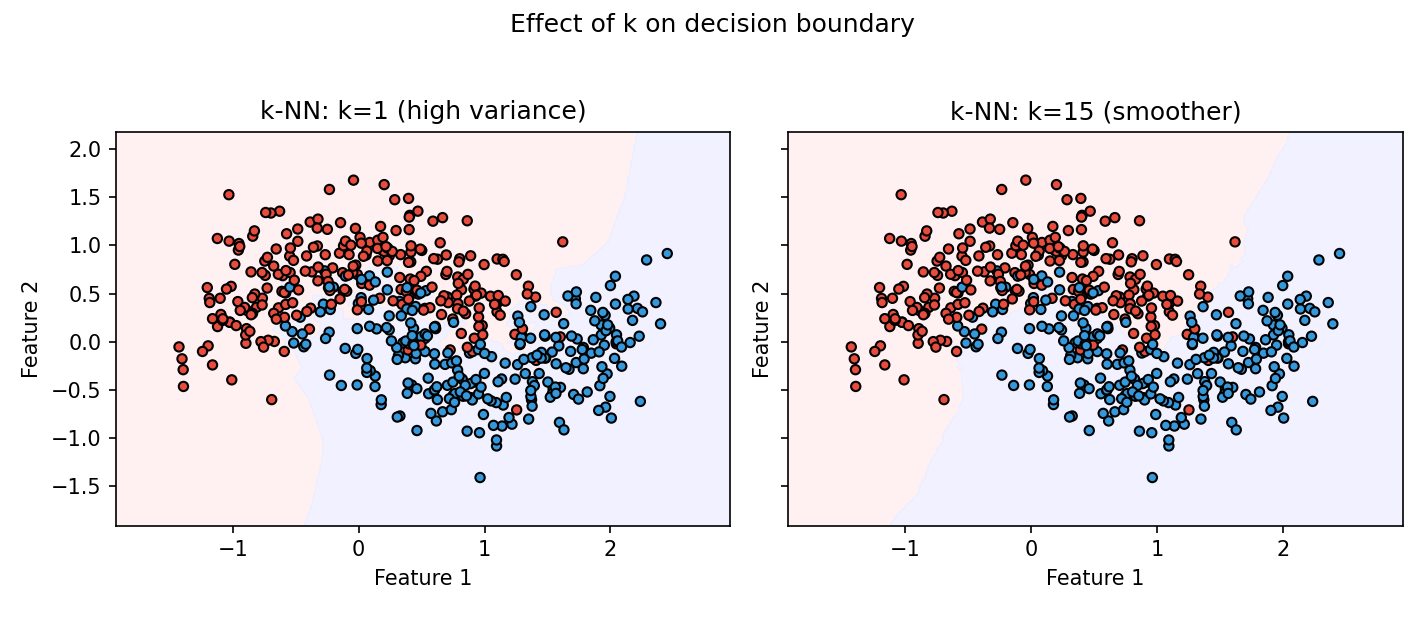
\includegraphics[width=0.95\linewidth]{knn_k_compare.png}
  \caption{Decision boundaries for different k (1 vs 15).}
  \label{fig:knn_k}
\end{figure}
\FloatBarrier

\begin{figure}[H]
  \centering
  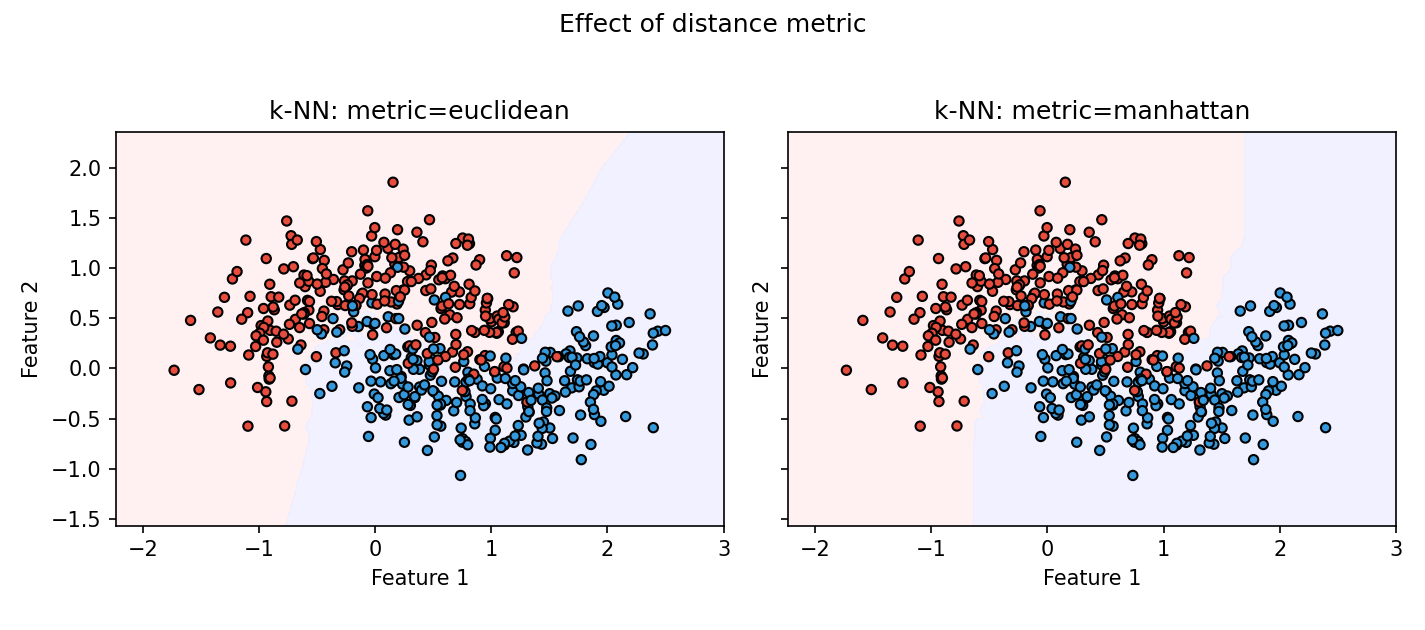
\includegraphics[width=0.95\linewidth]{knn_metric_compare.png}
  \caption{Effect of metric: Euclidean vs Manhattan.}
  \label{fig:knn_metric}
\end{figure}
\FloatBarrier

\begin{figure}[H]
  \centering
  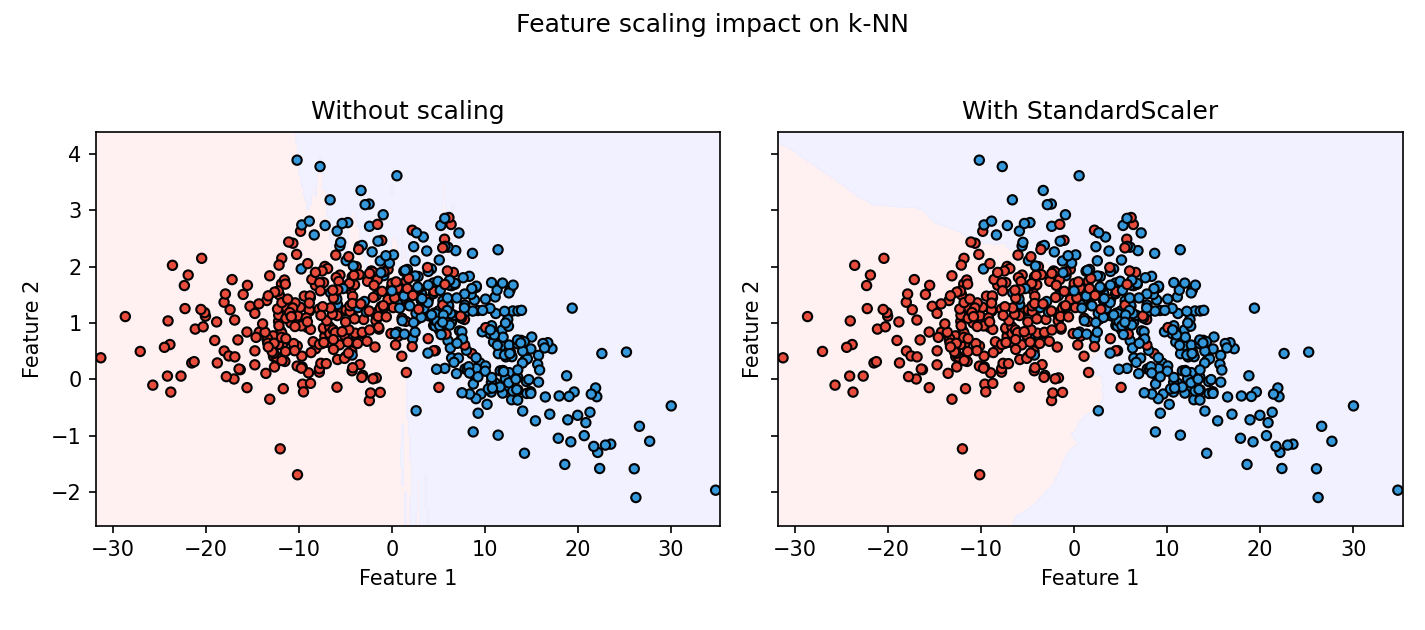
\includegraphics[width=0.95\linewidth]{knn_scaling_effect.png}
  \caption{Impact of feature scaling on decision boundary.}
  \label{fig:knn_scale}
\end{figure}
\FloatBarrier

\begin{figure}[H]
  \centering
  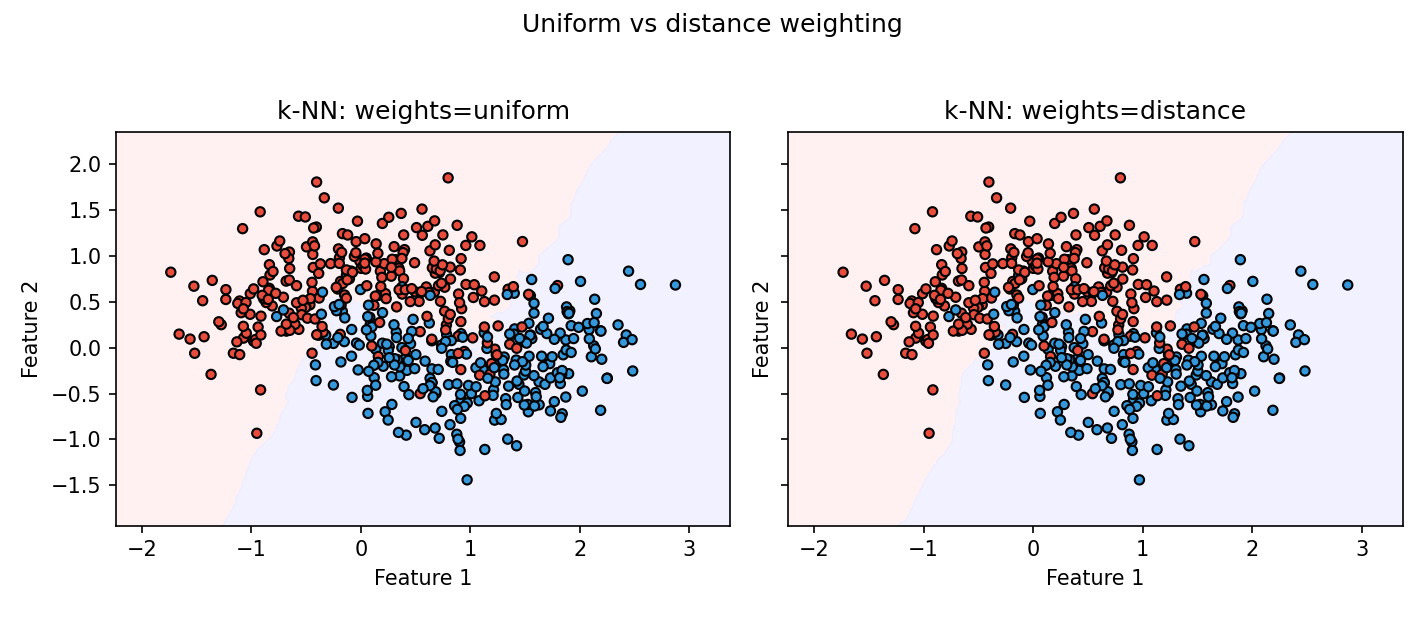
\includegraphics[width=0.95\linewidth]{knn_weight_compare.png}
  \caption{Uniform vs distance weighting in k-NN.}
  \label{fig:knn_weight}
\end{figure}
\FloatBarrier

\begin{figure}[H]
  \centering
  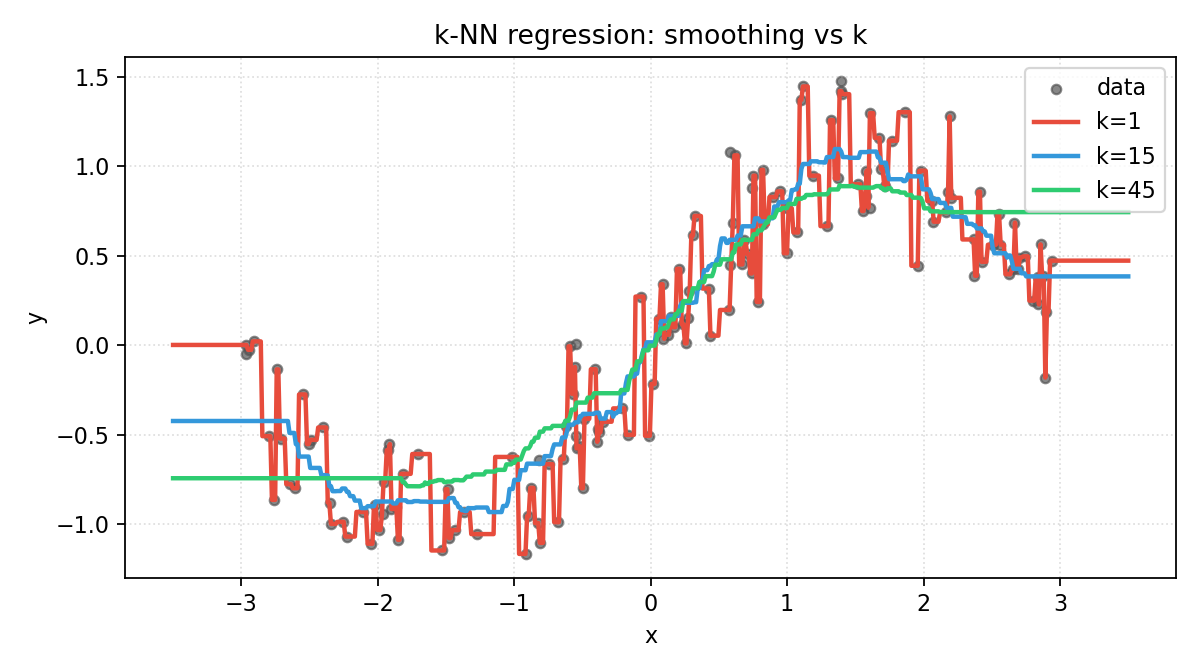
\includegraphics[width=0.85\linewidth]{knn_regression_curve.png}
  \caption{k-NN regression: smoothing effect as k increases.}
  \label{fig:knn_reg}
\end{figure}
\FloatBarrier

\section{Summary}
k-NN is a simple yet powerful baseline for both classification and regression when features are well-scaled and dimensionality is moderate. Select $k$, metric, and weighting via validation, and use scaling to ensure distances are meaningful.

\end{document}

